\chapter{Political Party Control and Intergovernmental Grants: a Panel Data Analysis}


\section{Introduction}
The strategic dynamics that exist between different tiers of governments have long been a focal point of fiscal federalism, particularly as they relate to the allocation of intergovernmental transfers \parencite{agrawal2022local,dahlby1996fiscal,gordon1983optimal}. In the fiscal federalism literature, these dynamics refers to how governments at different levels (e.g., federal, state, and local) elect to respond when their choices are influenced by another government's choices.  For example, a federal government that elects to transfer funds through a program that requires a certain level of matching from a subnational government (rather than through a general transfer program) may elicit the subnational government to accept or reject the grant offer. Given the presence of such dynamics, it is critical that they be considered in the design of intergovernmental transfer (IGT) programs \parencite{dahlby1996fiscal,gordon1983optimal}. A failure to properly consider how they affect fiscal behaviors can induce distortions that reduces the effectiveness of government spending, such as overspending by subnational governments or temporary adjustments in tax collections\parencite{bailey1998flypaper,inman2008flypaper,turnbull1998overspending}.

Academic interest in IGTs has produced a series of studies that offer insights into the complex negotiations and compromises that often characterize the IGT distribution process\parencite{chubb1985political,dixit1995redistributive,weingast1979rational}. Many of the investigations are based on game theory, which assumes that bargaining is carried out by rational players\parencite{banks2006general,baron1989bargaining,martin2018dividing}. However, a limitation of the game-theoretic approach is that it is often grounded in a rational choice paradigm that is at odds with the realities of the environment within which IGTs are distributed. To account for the complex reality of IGT, it is often necessary consider an array of additional factors that goes beyond assumptions of rationality and homogeneity\parencite{golden2008pork,milligan2005regional,petry1999electoral,tellier2006public}. \textcite{rosenstiel2021congressional}, for example,points to the need to consider factors such as partisan alignment and preferences for grant categories.

The purpose of this research is to add to the extant body of literature IGTs by examining how political party control affects federal government IGT distributions. Political party control remains a largely unexamined independent variable in analysis of IGT distributions in the US context. In the literature review that was conducted as part of this study, only two previous studies were found that explicitly addresses this topic\parencite{ansolabehere2002equal,ansolabehere2006party}. This research contributes to this stream by examining the influence of four distinct features of political party control are considered including (1) whether the federal government is unified, (2) the specific party in control, (3) political alignment across the federal and state governments, and (4) political competition across parties.


The analysis is conducted, using a fixed-effect regression model. Using panel data collected from 14 states, we find that political alignment significantly impacts the distribution of intergovernmental grants. Specifically, states with a unified government, where both the administrative and legislative branches at the state and federal levels are controlled by the same party, tend to experience variations in grant allocation. Republican-controlled states under a unified Republican federal government receive a reduced proportion of grants compared to states under bipartisan or Democratic control. Furthermore, our analysis indicates that swing states receive significantly less grant funding compared to their partisan counterparts in non-election years. This suggests a strategic behavior of federal governments, which may allocate resources not solely based on states' needs or economic conditions but also influenced by political considerations and party alignment.

These findings are important because of the scant research that surround the role of political party control in IGT distributions. Despite the presence of a relatively healthy body of theories stream of research that examine the influence of various stakeholders on budget outcomes, this independent variable remains largely unexamined in the US federal context\parencite{patashnik2000budgeting}.  It is also significant due to the significant role that politics play in the budget process. The budget is by many viewed as the prime expression of political preferences. \textcite{wildavsky2003new} viewed budgeting as the basic framework that makes decision-making in political environments possible.  He articulated the role of politics in budgeting as follows: “All Budgeting is about politics, most politics is about budgeting, and budgeting must therefore be understood as part of a political game.”

% Fiscal federalism has long been a focal point within the realm of public finance, particularly concerning the strategic dynamics between various tiers of government\parencite{gordon1983optimal,dahlby1996fiscal,agrawal2022local}.
% The allocation of intergovernmental transfers within this domain emerges as a critical area of inquiry, given its potential to profoundly influence governmental fiscal behavior and potentially lead to distortions\parencite{dahlby1996fiscal,gordon1983optimal}. For instance, these grants may induce overspending by subnational governments or stimulate/retard state governments' tax collection behavior\parencite{inman2008flypaper,bailey1998flypaper,turnbull1998overspending}. This paper seeks to unravel a fundamental question within the realm of American fiscal intergovernmental transfer: does the distribution of federal grants reflect the influence of party preferences and alignment between federal and state governments, as well as party attributes at the state level? These concerns pivot around the potential for federal bias favoring states with matching political affiliations, a significant inquiry given grants' role as 20\% of federal annual revenue \parencite{rosenstiel2021congressional}.


% Empirical investigation into the grants allocation of funds has delineated the complex negotiations and compromises that characterize grant distribution---a process described not merely as top-down decisions, but as federative conciliation \parencite{chubb1985political, 1976A, dixit1995redistributive}. Our focus narrows upon federal decision-making, assuming the compliance of subnational governments---a perspective less explored but critical in the intricate hierarchy of government interactions. The traditional investigation on the bargaining on federal level, often based on game theory, propose rational, identical players \parencite{baron1989bargaining, banks2006general, martin2018dividing}, but the diversity of stakeholders involved introduces an array of additional considerations\parencite{milligan2005regional, golden2008pork,tellier2006public, petry1999electoral}.
% Factors such as partisan alignment and preferences for grant categories are part of this multifaceted equation\parencite{rosenstiel2021congressional}, each contributing to the complex reality of grant distribution.

% This paper seeks to address gaps in the literature by empirically investigating the effects of party preference and alignment between federal and state governments, as well as state party affiliation, on intergovernmental transfer distribution. In addition, we want to distinguish whether the alignment effect, if it's significant, is due to the federal level's subjective favoritism towards states with similar party affiliations. By dissecting panel data spanning various states and political contexts, this paper will highlight how such political dynamics manifest in the actual allocation of federal funds.

% In Chapter 3, the dissertation takes a critical turn to explore the nuanced effects of political party control on the distribution and utilization of intergovernmental grants within the United States, a pivotal component of the fiscal federalism framework. This analysis directly supports the overarching aim of the dissertation to unravel the complex dynamics of fiscal interactions between central and subnational governments, by focusing on the political dimensions that underpin these interactions. By employing a panel data analysis over a 19-year period, this chapter sheds light on how political alignment and party control significantly influence the flow of intergovernmental transfers, adding a critical layer of understanding to the strategic fiscal behaviors of governments within the federal system. This exploration not only enhances our comprehension of fiscal federalism's theoretical and practical applications but also underscores the importance of political considerations in the design and execution of fiscal policies. As such, the findings from this chapter contribute to a more nuanced understanding of fiscal federalism and intergovernmental transfer, enriching the dissertation's holistic examination of governmental fiscal strategies and their implications for public service delivery across different tiers of government.

% Following this introduction, a comprehensive overview of the grant distribution rules in the United States will set the platform for our narrative. We will then proceed with a robust literature review to carve out the missing pieces in the existing body of research. Our research questions and hypotheses will be postulated with precision and academic rigor, subsequently leading to a dialogue on our research methodology and an analysis of the findings in pursuit of academic and practical enlightenment.


\section{Intergovernmental Grants: A Background}
Consistent with recent trends in the academic literature\parencite{abbott2012intergovernmental,akai2019role,lago2024effects}, this paper uses the terms intergovernmental transfers and grants interchangeably to depict fiscal handovers from one government tier to another. In federal systems, such handovers serve as a multifunctional fiscal instrument, designed to not only instill spending in national-priority sectors but also to harmonize fiscal imbalances across regions. Intergovernmental transfers are therefore often viewed as being instrumental in strengthening subnational entities, and in addressing regional inequities, including vertical disparities rooted in structural differences and horizontal inequities emanating from diverse fiscal capacities and expenditure requirements of sub national jurisdictions.

The process through which intergovernmental transfers are distributed is often depicted through the lenses of a game-theoretic bargaining game. Such a framework is helpful because it captures the strategic dynamics that surround the distribution of intergovernmental grants in democratic environments, and that continues to be a focal point of fiscal federalism\parencite{agrawal2022local,dahlby1996fiscal,gordon1983optimal}. These dynamics refers to how governments at different levels (e.g., federal, state, and local) elect to respond when their choices are influenced by another government's choices.  For example, a federal government that elects to transfer funds through a categorical transfer program that requires a certain level of matching from a subnational government (rather than through a general transfer program) may influence whether subnational government elects to accept or reject the grant offer. Extant research show that consideration of strategic dynamics is a critical determinant of the success of intergovernmental grants (IG)\parencite{dahlby1996fiscal,gordon1983optimal}. If not accounted for, they may cause fiscal behaviors that reduces the effectiveness of government spending, such as overspending by subnational governments or temporary adjustments in tax collections\parencite{bailey1998flypaper,inman2008flypaper,turnbull1998overspending}.

Over time, important advances have been made to further refine these frameworks in ways that that make them more capable of capturing the strategic dynamics that surround intergovernmental transfers. A seminal contribution in this regard is a paper by \textcite{baron1989bargaining}, which laid the foundation for much of the subsequent work. It depicts the distribution of grants as a bargaining game among different decision-making groups, when one participant in the game is the decision-making institution, such a congress or a specific committee. \textcite{baron1989bargaining} bargaining framework is built around four rules that are regarded as crucial to simulations of the bargaining process that determines grants distribution. These include the recognition rule, voting rule, amendment rule, and money-distribution rule.


\begin{enumerate}
    \item The recognition rule determines how to select the agenda setter that make the initial proposal. In the extant literature, most simulations are grounded on the random recognition rule, which assumes that members of the decision-making institution have equal probabilities of being chosen to make the initial proposal\parencite{anesi2015bargaining, diermeier2011legislative,kalandrakis2004three,rosenstiel2021congressional}.
    \item The voting rule establishes the standard for passing the proposal, with the majority rule and unanimous voting rule being common assumptions\parencite{baron1989bargaining}.
    \item The amendment rule places constraints on making amendments, ranging from the closed rule (allowing no amendments) to the open rule (allowing any and all germane amendments).
    \item The grants-type rule determines how grants could be manipulated by decision-making institutions, with some scholars assuming direct decisions on the number of receivers, referred to as "earmarks" spending models.
\end{enumerate}

\textcite{baron1989bargaining}'s foundational paper also established several important assumptions that accompanied their framework, such as random recognition, majority voting rule, and earmarks rule. Their work, along with a subsequent study by \textcite{banks2006general}, offers three key insights. First, it demonstrates that legislators with agenda-setting power tend to receive a disproportionate share of funding. Second, it demonstrates that, when in a state of equilibrium, funds flow only to legislators in the winning coalition, with no funds allocated to those outside of it. Third, they found that when proposals are brought up under a closed rule, the winning coalition is minimized, leading to the maximization of benefits for the members of the winning coalition.

More recently, a study by \textcite{martin2018dividing} added to \textcite{baron1989bargaining}'s framework by modifying the assumptions of the model, including its heavy reliance on “earmarks.” Martin's modified model placed limits on decision-makers' power to determine the factors in the formula rather than the specific numbers. This modification generates a model that is more closely aligned with the realities of political and administrative life. It also produces two conclusions that differs from those of Baron and Ferejohn's model. First, in contrast to the original model, Martin's model predicts oversized winning coalitions and the emergence of persistent winning blocs. Additionally, \textcite{martin2018dividing} demonstrates that when bargaining occurs over a low-dimensional formula  ,  (i.e, less than five variables included in the formula) legislators have limited ability to target funds to specific districts; a prediction supported by empirical evidence. For instance, Martin analyzed existing formula grants and found that 95\% of the formulas have fewer than 5 variables, indicating limited bargaining dimensions for members. Consequently, some jurisdictions can be free riders, even if they are not part of the winning coalition. Based on these findings, Martin predicts a positive distribution outside the winning coalition.

However, there are several limitations with applying game-theoretic models to explain IGT distributions. Many of these arise from the fact that they often are grounded in a rational choice paradigm that is at odds with the realities of the environment within which IGTs are distributed. To account for the complex reality of IGT, it is often necessary consider an array of additional factors that goes beyond assumptions of rationality and homogeneity \parencite{golden2008pork,milligan2005regional,petry1999electoral,tellier2006public}. \textcite{rosenstiel2021congressional}, for example, points to the need to consider factors such as partisan alignment and preferences for grant categories.

\section{Political Party Control and IGT Distributions: Literature Review }

As noted in the introduction, the purpose of this paper is to examine how the distribution of political party control affects IGT distributions in the US federal budgetary context.  In the literature review that was conducted as part of this study, two previous studies were found that explicitly addresses this topic\parencite{ansolabehere2002equal,ansolabehere2006party}. Both studies are confined to examining aspects of party control on intergovernmental distributions from state governments to counties. The earlier study \parencite{ansolabehere2002equal} examined the distribution of funds from money by states to counties. Using cross-sectional analysis, it showed that the proportion of legislative seats per person was positively related to the amount of transfers a county received from the state per person. The more recent study \parencite{ansolabehere2006party} examined the distributive expenditures across counties in US states over a 40-year period. The study shows that (1) counties that traditionally support (in terms of vote share) the governing party tend to receive larger shares of state transfers, and (2) that the distribution of IGTs tends to follow the direction of the shifts across governing parties.

\textcite{borck2003political} investigates the impact of political factors on the distribution of intergovernmental grants through modeling and empirical data analysis. The core of the research focuses on local government officials lobbying the central government to secure more funding. The article proposes that lobbying costs increase with the geographic and political distance from the central government, theoretically leading to a decrease in grant allocation with increased distance. Their Empirical analysis using county-level data from California finds a negative correlation between grant allocation and geographic distance, aligning with the hypothesized political access costs. Furthermore, the study observes that regions politically aligned with the central government tend to receive more funding. During the response of Covid-19 pandemic in America, \textcite{terman2015performance,terman2020getting,terman2015improving,terman2022even}'s series of studies extensively examines how political alignment, partisan relations, and administrative capabilities impact the distribution and efficiency of federal funds. Her findings highlight the significant role of partisan congruence in enhancing the effectiveness of policy implementation during crises like the COVID-19 pandemic.

Similar analysis is also found outside America, \textcite{sole2008effects}explore the influence of partisan alignment with upper-level governments on local funding in Spain, demonstrating that local units aligned with higher government tiers tend to receive more funding.   These research highlights the significance of political motives in the distribution of intergovernmental grants, showing that the actual allocation of government funding can deviate from ideal efficiency levels due to political influences, even in areas with evident public service spillover benefits.

Besides, a series of studies were produced in the 1970s and 1980s that examined whether party control was related to increases in spending on programs that were ideologically preferred by a particular party. \textcite{carlino2023partisanship} find that Republican governors are less inclined than their Democratic counterparts to spend on federal intergovernmental transfers. As a result, states led by Republicans tend to have lower debt levels, delayed taxation, and initially lower economic activity. Overall,  At the state level,
these studies offer limited evidence in support of such influence \parencite{fry1970politics,winters1976party,plotnick1985politico,  lowery1987distribution, marquette1981competition, plotnick1990party}. However, at the federal level a stronger correlation was found \parencite{owens1984federal,browning1973geography,levitt1995political, ritt1976committee,kiewiet2002here, ansolabehere2006party}. In addition to this latter finding, this stream of research is valuable in that it offers insights into how
to operationalize studies of political control (see methods section).

Explicitly stated, this research adds to the above literature by examining the role of political party control in IGT distributions from the US federal government to the states. In the U.S. federal context, intergovernmental grants are typically classified along two dimensions \parencite{clemens2023intergovernmental,dilger2015federal}, including (1) the level of control that federal agencies exercise in terms of directing how grant funds are used by a subnational government, and (2) the methodologies employed to determine grant amounts or grant shares. The former dimension can be used to categorize three common grant types including categorical grants, block grants and general revenue sharing grants. Among these grant types, categorical grants provide federal agencies with the highest level of control and influence over how state and local government spend awarded funds. They often come attached with language that narrowly defines the purposes for which a subnational government may spend distributed funds.

Block grants signify the distribution of funds that are earmarked for a specific program or project, rather than a narrowly defined spending purpose. Federal agencies exercise less control over block grant programs, compared to categorical grant programs, given that they are earmarked at the program level. For the recipient, they constitute a relatively flexible pool of funds permitting the recipient subnational government to tailor the design and implementation of programs in response to identified regional needs \parencite{finegold2004block}.

Finally, general revenue sharing grants refer to grants that are apportioned to subnational governments, using a part of a central government's tax revenues. Sometimes referred to as unconditional grants, they impose very few restrictions on recipient subnational governments. They are distributed to subnational governments through some form of pre-defined formula, defined by law, where the receiving units may or may not be required to match the amounts received\parencite{larkey2015evaluating}. Given that general revenue sharing grants are based on a predefined formula, they extend very limited opportunities for federal agencies to control or influence the distribution of federal funds.


The second dimension mentioned above is the methodologies employed to determine grant amounts or grant shares. Based on this dimension, relevant grant types include project grants, formula grants and reimbursement grants. Project grants refer to grant funds distributed to fund particular projects or deliverables. This grant type is awarded through a competitive process, encouraging states to
propose and execute exemplary projects\parencite{dilger2015federal}.Formula grants are noncompetitive grants that are allocated to subnational governments based on a pre-defined formula. Such formulas often consider a variety of economic and social characteristics within a jurisdiction\parencite{huffman2006formula}. Whether formula grants eliminates political motives in resource distribution is unclear yet. \textcite{banful2011formula} delves into whether Ghana's implementation of the formula-based District Assemblies Common Fund (DACF) effectively eliminates political motivations in intergovernmental grants. The findings indicate that despite the formula-based allocation mechanism, political factors still play a significant role in the distribution of the District Assemblies Common Fund. Especially around elections, the government tends to allocate more funds to key or politically sensitive areas. This suggests that despite the system's design for fairness, political motivations can still influence the actual distribution of resources.   Finally, reimbursement grants reimburse state and local governments for a portion of their expenditures on specific programs. They are awarded using open-ended and closed-ended matching grant variations.


In this paper we propose that political party control is channeled into IGT distributions through the level of control that central government agency officials and legislators exercise over such distributions. At the administrative level, this level of control is defined through the laws that accompanies different types of grant programs. For example, non-discretionary grant programs, where allocations are determined by a set formula, offers limited opportunities for federal agencies to control and influence distributions. On the other end, categorical grant programs often extend substantial control to the administrative agencies.

The previously mentioned dimensions used to classify intergovernmental grants provide a useful framework for depicting the level of discretion that accompanies different grant types. Figure \ref{grantstype} depicts the different grant type possibilities, using a two-dimensional matrix. It suggests that the control that federal agencies and administrators exercise over grant distributions reaches its zenith with categorical project grants. This grant form extends substantial authority to the federal agency in terms selecting recipients and determining grant amounts. Reimbursement grants, while less directly controlled, provides some opportunities for federal agencies to steering benefits towards preferred states.

According to the Congressional Research Service, federal agencies distribute federal funds via close to 600 federal grant programs\parencite{dilger2015federal}. Close to 70 percent of these programs is some form of project grant\parencite{dilger2015federal}. Hence, a substantial portion of intergovernmental grants are distributed through grant programs where federal agencies exercises substantial levels of control over grant distributions.

At the legislative level, the influence over grant distributions occurs at the time when legislators establish the basic parameters that guides grant distribution for the various programs. For example, the selection criteria embedded in formula grants can be oriented to favor certain constituencies that reflects legislators' preferences\footnote{While the selection criteria embedded in formula grants can be oriented to favor certain constituencies, such criteria would reflect legislators' preferences at a time that precede the distribution, rather than preferences during the distribution year, presuming these do not coincide.}. It may also occur indirectly through pressure that legislators impose on administrative agencies.

\section{Hypothesis}

To examine the general proposition that political party control influence IGT distributions, this study considers four factors that we argue captures important aspects of party control. These include (1) whether the federal government is unified, (2) the specific party in control, (3) political alignment across the federal and state governments, and (4) political competition across parties. These factors were included because they have been identified as features of political party control in previous research.

The first feature of political party control that is considered is whether the federal government is unified or not. A unified government is characterized by the alignment of the administrative branch and legislative branch at the federal level under the same political party. A unified government is a feature of political party control, given that  it reduces the need for political compromises across parties. \textcite{coleman1999unified} states that a unified government is productive in public policy outcome. Given this, such alignment is argued to result in higher overall spending. Explicitly stated, the first hypothesis is:

\textbf{Hypothesis 1: A unified federal government is positively associated with higher overall IGT spending.}

The second feature of political party control that is considered is the specific party in control. The Democratic and Republican parties are presumed to exhibit distinct preferences regarding the scale of IGTs\parencite{weaver2010paths,winters1976party}. However, it is challenging
to interpret these differences in party preferences toward IGTs. The Democratic Party tends to favor a larger and more centralized government and the republican party tends to favor a smaller and more decentralized government. The Democratic party's preference toward a larger government suggests a positive association with IGT spending. At the same time, the Republican party's preference for decentralization goes hand in hand with IGTs.Consequently, these contrasting preferences lead to divergent conclusions. Given this, the second hypothesis is:

\textbf{Hypothesis 2: Political party color is related to the level of IGT spending.}

The third feature of political party control is the level of political alignment across the federal and state governments. Research by \textcite{ansolabehere2006party} show that hat counties that traditionally have supported the governing party (in terms of vote share) receive a larger share of
state transfers to local government. They also find evidence that counties with greater legislative seats per person receive more transfer payments from state governments\parencite{ansolabehere2002equal}.In this research, we test whether a similar effect is present in the context of IGT transfers from the federal government to state governments. Explicitly stated, we hypothesize that:


\textbf{Hypothesis 3: The level of political party alignment across the federal and state governments is positively related to IGT distributions.}

The final feature of political party control that is considered is whether a state is a battle ground state or not. The federal government, driven by the motivation to secure election or reelection, is inclined to allocate resources and provide additional public goods to states that significantly influence electoral outcomes. This strategic allocation is aimed at accruing political credits. \textcite{veiga2013intergovernmental} reveal how intergovernmental fiscal transfers are utilized as political tools during electoral cycles, with increased transfers to certain regions to boost political support in election years. \textcite{dahlberg2002vote} analyze the strategic allocation of intergovernmental grants in Sweden before elections, supporting the Lindbeck-Weibull/Dixit-Londregan model that governments allocate more funds to areas with a high number of swing voters.Therefore, we argue that swing states are more likely to secure IGTs. Explicitly stated, the final hypothesis is:

\textbf{Hypothesis 4: Battle ground states are more likely to secure IGTs compared to non-battle ground states.}

%%%%%%%%%%%%%%%%%%%%%%%%%%%%%%%%%%%%%%%%%%%%

\section{Research Approach}


To test the above hypotheses, we undertook a two-step analytical approach. The first step was conducted using a principal components analysis (PCA). This step was conducted for purposes of establishing the extent to which IGT distributions are driven by shared economic and social
attributes among same-party states. This step was added to the analysis as a result of \textcite{martin2018dividing} observation that biases in IGT distributions may partially be driven by shared economic and
social attributes among same-party states, given that such attributes often determine grant distributions established by formulas. The second step centered on testing the above four hypotheses. Toward this end, we conducted a fixed regression analysis based on the panel data of states in America.


% In the context of this study, the disparities in the distribution of intergovernmental transfers and their link to political party attributes may stem from two distinct reasons. Firstly, the alliance effect, which is subjective in nature, suggests that higher-level governments prefer to allocate more funds to lower-level governments that share the same political party affiliation. The second reason revolves around a preference for certain economic and social development policies by higher-level governments, thereby benefiting all lower-level governments that exhibit specific economic and social characteristics. Often, these shared economic and social attributes align with political party affiliations. To achieve the research objective, namely, to ascertain the presence of the first reason, it is imperative to examine the validity of the second reason before employing regression analysis to investigate the relationship between disparities in transfer payments and political party attributes. If the influence of the second reason holds, meticulous control is necessary to disentangle its effects from those attributed to alliance effects. Thus, the application of Principal Component Analysis (PCA) prior to regression analysis serves a crucial role. It allows for the investigation into whether variations in transfer payments are merely a reflection of economic and social characteristic preferences, which coincidentally align with political affiliations. This step is fundamental in ensuring that our analysis accurately identifies the influence of subjective political alliances, free from the confounding impact of shared economic and social traits across different political administrations.


\subsection{Step 1: Principle Components (PCA) Analysis}

In the context of this study, disparities in the distribution of IGTs may stem from two distinct effects. The first effect, which we refer to as the alliance effect, is assumed to arise from a higherlevel government's preference toward allocating funds to lower-level governments that share its political party affiliation. The political party control features that are examined in this research are assumed to generate alliance effects. The second effect, which we refer to as the preference effect arises from a higher-level government's preferences toward funding certain economic and social development policies. In terms of IGT distributions, this effect benefits lower-level governments
that exhibit certain economic and social characteristics. These shared economic and social attributes may align with political party affiliations. More specifically, numerous American and international studies have provided evidence indicating that factors such as economic structure and economic
conditions influence political affiliation. Therefore, it is plausible to infer that the reverse logic holds true: regions governed by the same political party may also share similar economic and social structures\parencite{Alan2009Partisanship,anderson2006economic,weatherford1978economic}. Given this, it becomes important to examine the potential influence of the preference effect, before employing regression analysis to investigate the relationship between disparities in transfer payments and political party attributes. If
it is established that the preference effect is prevalent, additional controls are necessary to disentangle its effects from those attributed to alliance effects. Hence, the application of PCA prior to regression analysis serves this crucial role. That is, it allows us to determine whether variations in
transfer payments are merely a reflection of economic and social characteristics that coincidentally align with political affiliations.

A PCA is a statistical technique that allows researchers to simplify the complexity of highdimensional data while retaining trends and patterns. It allows for this by transforming the original variables into a new set of uncorrelated variables, referred to as the principal components. These
principal components are ordered so that the first few variables retain most of the variation present in the original variables. PCA is particularly useful when analyzing data with numerous interrelated variables to identify underlying structures within the data. For purposes of this research, it allows us
to reduce the dimensionality of data, and improves interpretability while minimizing information loss. By focusing on the principal components with the highest variances, it allows us to discern the most significant patterns and relationships within the data.

It is useful to apply when analyzing data with numerous interrelated variables to identify underlying structures within the data. This method is particularly beneficial in reducing the dimensionality of data, improving interpretability while minimizing information loss. By focusing on the principal components with the highest variances, researchers can discern the most significant patterns and relationships within the data.

The primary aim of the PCA that was conducted as part of this study was to distill economic and social characteristics of states into a manageable number of components that could reveal potential clustering by political affiliation. To accomplish this, we (1) standardized the dataset to ensure each
variable contributed equally to the analysis; (2) computed a covariance matrix to identify relationships between variables; and (3) extracted eigenvalues and eigenvectors to determine the principal components. Following these three steps, the resulting components were analyzed to determine the extent to which they captured the variance in our data, thereby guiding us in determining the number of dimensions needed for further analysis. This latter step was crucial for isolating the shared economic and social attributes among same-party states. It provided a foundation for understanding how these attributes might influence IGT distributions beyond the surface level of political alignments and preferences.


\subsubsection{Data and variables for PCA Analysis}
The primary variables required mainly consist of economic and social characteristics at the state level, with particular emphasis on variables frequently appearing in transfer payment formulas. Additionally, as this article specifically focuses on the economic and social commonalities among states governed by the same political party, a grouped sampling method was adopted for selecting sample states. All states were categorized into traditional Democratic states, traditional Republican states, and traditional swing states. Within each group, 5-6 states were randomly selected as samples. The economic and social variables of all selected sample states were then analyzed for annual changes from 2000 to 2019, thus forming a panel dataset.

The state grouping method relies on two primary criteria: historical presidential election outcomes and their corresponding winning percentages, a methodology delineated in \textcite{beachler2015presidential}. Democratic and Republican states are characterized as those consistently favoring a particular party in presidential elections since 1984, where the winning rates surpass 58\%. Swing states are recognized as those that have alternated between parties in selecting presidents, with winning rates falling below 58\%. The states encompassed within the analysis are enumerated in Table \ref{Table 2.3}.


The social and economic characteristics commonly included in the formula for intergovernmental transfers encompass population, working-age population weight, median household income, unemployment rate, road mileage, and GDP per capita \parencite{dilger2015federal}. I gathered all factors mentioned in \Textcite{dilger2015federal}'s study for the sampled states. Additionally, I referenced major intergovernmental transfer programs such as Medicaid, the Title I-A education program, Temporary Assistance for Needy Families (TANF), Section 8 Housing Choice Vouchers, and the Community Development Block Grant (CDBG) to comprehensively collect factors. To ensure data convenience for regression and enhance data visualization, I performed appropriate operations. The collected characteristics and data sources are detailed in Table \ref{Table 2.4}.%%%%%%chatgpt checked%%%%%


\subsubsection{PCA Process and Results}

Issues of correlation across the collected variables are evident. For example, the weight of the working-age population and the unemployment rate are highly interdependent. Moreover, higher population levels inherently correspond to increased usage of public roads. This observation is further corroborated by the correlation heatmap, depicted in Figure \ref{heatmap},which indicates a certain degree of correlation among the variables. As such, we conclude that PCA is needed to reduce data dimensionality and mitigate issues of multicollinearity.%%%%%chatgpt checked%%%%%

% \begin{figure}
%     \centering
%     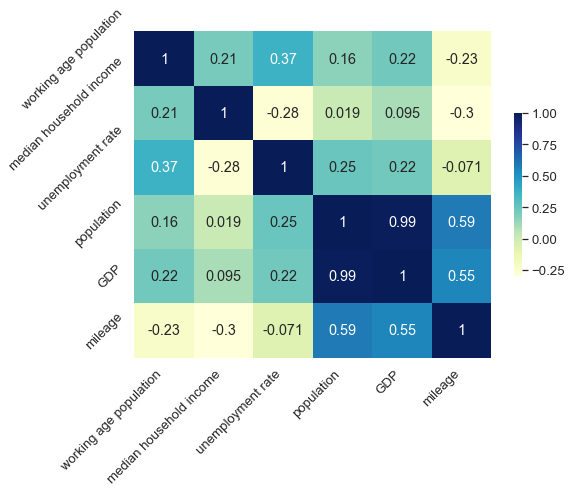
\includegraphics[scale=0.7]{Chapter-3/Figures/heatmap.png}
%     \caption[Heatmap of the Social Characteristics]{Heatmap of the Social Characteristics
%         \texttt{} }
%     \label{heatmap}
% \end{figure}

To address the first question, the apparent hindrance lies in the difficulty of directly assessing the similarity of jurisdictions in social and economic characteristics. To overcome this challenge, I employed Principal Components Analysis (PCA) to reduce data dimensionality and mitigate issues of multicollinearity. This approach aims to determine whether the reduced-dimension data exhibit cluster distribution or scattered distribution.

The results of the PCA variance analysis, as depicted in the figure, reveal that the first two dimensions encapsulate 67\% of the information, while the first three dimensions account for 87\% of the information.
% \begin{figure}[H]
%     \centering  %居中
%     \subfigure[Histgram]{   %第一张子图
%         \begin{minipage}{7cm}
%             \centering    %子图居中
%             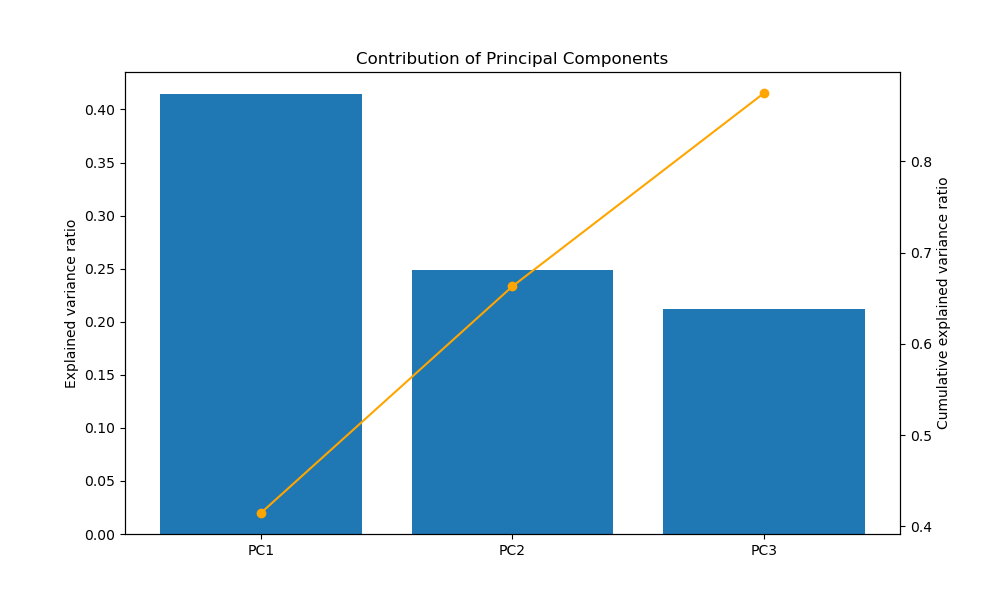
\includegraphics[scale=0.2]{Chapter-3/Figures/contribution.png}  %以pic.jpg的0.5倍大小输出
%         \end{minipage}
%     }
%     \subfigure[Line]{ %第二张子图
%         \begin{minipage}{7cm}
%             \centering    %子图居中
%             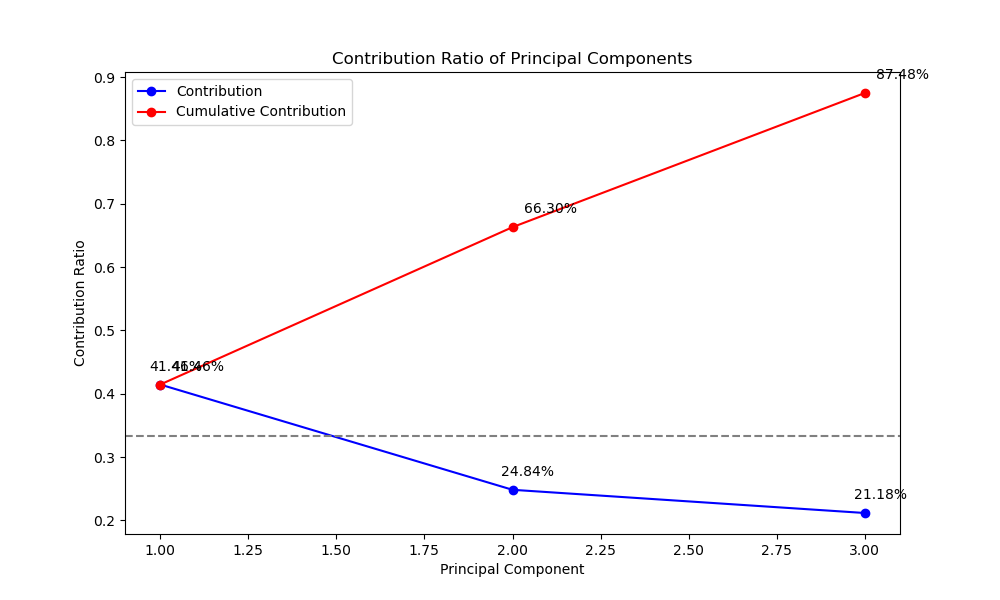
\includegraphics[scale=0.2]{Chapter-3/Figures/contribution2.png}%以pic.jpg的0.5倍大小输出
%         \end{minipage}
%     }
%     \caption[Principle Components Contribution]{Principle Components Contribution}    %大图名称
%     \label{principlecomponentcontribution}    %图片引用标记
% \end{figure}

Consequently, Principal Components Analysis (PCA) was employed to reduce the data into two and three dimensions separately. By retaining the two and three principal components with the highest information content, it became feasible to compare the characteristics between jurisdictions.

The results of the PCA variance analysis reveals that the first two components capture 67\% of the information, and the first three components capture 87\% of the information. Given this, we employed PCA to reduce data into two and three dimensions, respectively. By retaining the principal components with the highest information content, we were able to compare the
characteristics between jurisdictions, using scatter plot diagrams (see Figure \ref{Figure 2.2}). In both the two-dimensional and three-dimensional scatter plot diagrams, the red, blue, and green points exhibit distinct distributions, with each color forming its own cluster.
% \begin{figure}[H]
%     \centering  %居中
%     \subfigure[Histgram]{   %第一张子图
%         \begin{minipage}{7cm}
%             \centering    %子图居中
%             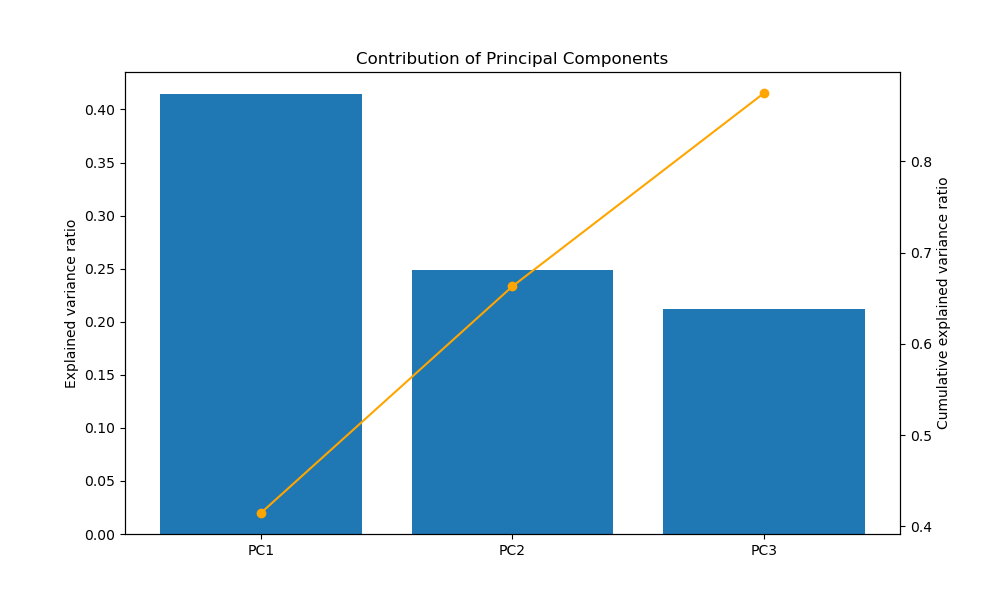
\includegraphics[scale=0.2]{Chapter-3/Figures/contribution.png}  %以pic.jpg的0.5倍大小输出
%         \end{minipage}
%     }
%     \subfigure[Line]{ %第二张子图
%         \begin{minipage}{7cm}
%             \centering    %子图居中
%             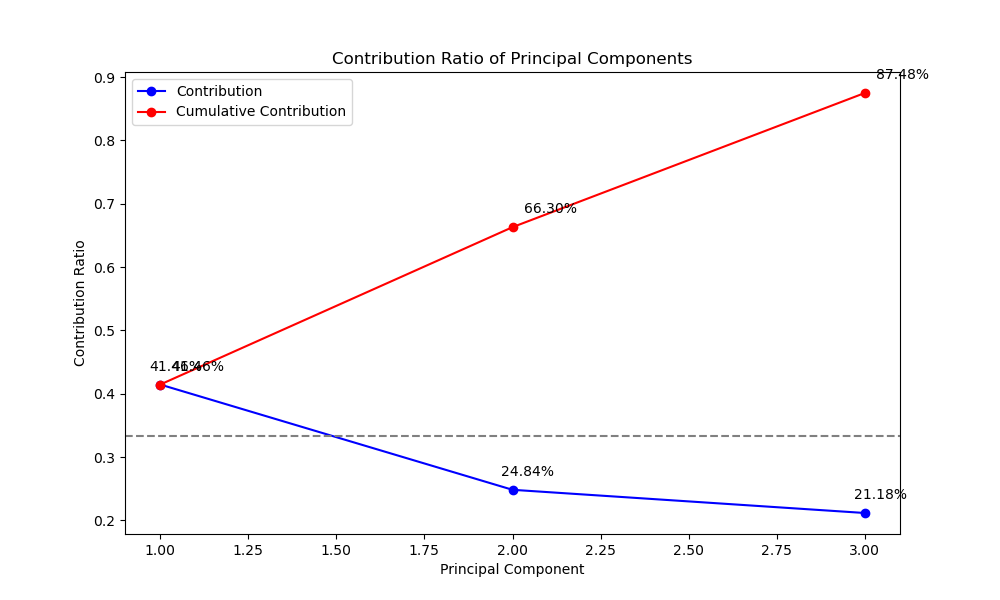
\includegraphics[scale=0.2]{Chapter-3/Figures/contribution2.png}%以pic.jpg的0.5倍大小输出
%         \end{minipage}
%     }
%     \caption[Principle Components Contribution]{Principle Components Contribution}    %大图名称
%     \label{principlecomponentcontribution}    %图片引用标记
% \end{figure}
Although the reduced components lack specific economic meaning, it is notable that many state characteristics exhibit a cluster distribution. Both the two-dimensional and three three-dimensional scatter plot diagrams suggests that states governed by the same political party share similar economic and social characteristics. This is notably different from states governed by other parties. In summary, therefore, the PCA indicate a high level of cohesion within states governed by the same party in terms of their economic and social characteristics, while significant differences exist between states governed by different parties. This finding is consistent with \Textcite{martin2018dividing}'s proposition that jurisdictions with similar features may have winners emerging from the bargaining game that are free riders, thereby predicting the outflow of funds from the winning coalition.

The scatter plot diagrams also show that republican states, democratic states, and swing states exhibit distinct cluster distributions in their respective areas. In the 2D plot presented, red and blue dots are situated on opposing sides, with swing states occupying the intermediary position. This
configuration implies that any modifications to the grant formula favoring one party inflicts significant harm to the other. This observation may reflect opposition between the two parties during legislative bargaining, while swing states remain relatively indifferent. The distinctive nature of swing states is further highlighted in the 3D scatter plot, where green dots do not align. While it may not be surprising that traditional Republican states share similar social characteristics, the 3D scatter plot provides an alternative perspective on fiscal collective behavior within the Republican party. It raises the question of whether those who take part in the bargaining process act based on
their political status or advocate for the benefits of the jurisdiction they represent. Hence, the preference effect may be mixed with the “free-rider” effect. To evaluate the effect of party preference, alignment and structure of different branches, the "free rider" effect should be carefully controlled.

In summary, the apparent collective alliance among ostensibly similar political parties may be the result from the similarities in economic and social characteristics of states governed by the same political party. Hence, the PCA results underscores the need to establish a micro-foundation for any
collective political behavior within a party. That is, it is essential to analyze the motivations of individual members rather than attributing it to collective group behavior.

\subsection{Step 2: Fixed Effect Regression Analysis}

To test the above four hypotheses, we employed a fixed effect regression analysis, a method ideally suited for panel data where multiple observations from the same entities (in this case, states) are observed over time. This approach allows us to control for unobserved heterogeneity that could bias our results, meaning it accounts for inherent characteristics of each state that do not change over time or are constant for each state across the study period. By focusing on the variations within each state, rather than between states, fixed effect models provide a more accurate estimation of the impact of political alignment and party preference on IGT distributions.

In preparation for the fixed effect regression analysis, we structured our panel dataset to include state-specific observations across multiple years, capturing the annual total amounts of IGT received by each state, along with the political party alignments at both the state and federal levels.
The model included dummy variables for each state to capture unobserved, time-invariant characteristics. Independent variables of interest were lagged to address potential endogeneity concerns, ensuring that we capture the effect of prior political conditions on current IGT distributions. The regression equation was also augmented with time dummies to control for year-specific
effects that might influence all states similarly, such as national economic conditions or federal policy changes. Standard errors were clustered at the state level to account for serial correlation within states over time. This comprehensive approach allowed us to examine the above hypotheses, while controlling for both observed and unobserved factors that could skew the results.


\subsubsection{Data and Variables for Regression}

Similar to the PCA, stratified sampling is also adopted. The sample states used when conducting the regression analysis are therefore the same as the ones used for the PCA. These were grouped into traditional Republican states, traditional Democratic states, and swing states. The dependent variable in the regression model is the annual total IGT amount received by state $i$. This variable
was operationalized though logarithmic transformation.

The independent variables include $c$, which is a dummy variable that represents alignment combination and $p$, which represent partisanship. More specifically, the dummy variable $c$ represents the party distribution combination in the administrative and legislative branches across
federal and state levels. Three key factors determine the nature of $c$: the governmental level, branch, and part. As depicted in Table \ref{Table 2.6},these factors can be presented in a $2\times2$ table with two
branches and two levels, resulting in four sectors. These sectors are denoted as $u_1, u_2, s_1, s_2$. Each sector has two possible parties in control, namely the Democratic party "$d$" and the Republican party "$r$".
% \end{table}%

In this study, the majority in the House of Representatives defines the partisan composition of the legislative branch, given its pivotal role in the budget-making process. The partisan composition of the administrative branch is determined by the partisan affiliation of the administrative leader, who
could be the president or governor. There are 16 combinations in $c$:

$$(r, r, r, r), (r, r, r, d), (r, r, d, r), (r, r, d, d), (r, d, r, r), (r, d, r, d), (r, d, d, r), (r, d, d, d)$$\\$$(d, r, r, r), (d, r, r, d), (d, r, d, r), (d, r, d, d), (d, d, r, r), (d, d, r, d), (d, d, d, r), (d, d, d, d) $$

We employ $c_1, c_2, . . . c_{16}$ to denote the 16 distinct combinations. In the regression analysis, only fifteen combinations are retained, with the omission of the first combination $c_1 = (r, r, r, r)$ to mitigate multicollinearity issues. $c_1$ serves as the benchmark in the regression model.


In the regression analysis, I incorporate a 1-time period lag of $c$ as an independent variable. The rationale behind this is that the general decision-making process is time-consuming, implying that the effect of a specific party combination $c$ should not be significant in the current year.

Regarding the dummy variable $p$, we gathered longitudinal data for three distinct types of states based on their political affiliations, including traditional Democratic states, Republican states, and
swing states. The 14 states are categorized into three groups. The first group constitutes the traditional Republican states, often referred to as the “red wall states.” We refer to this group as $p = 1$ The second group (referred to as $p = 2$) comprises traditional Democratic states, also known as
the “blue wall states.”. The third group (referred to as $p = 3$) represents swing states, commonly referred to as the “battleground states.”

The control variables encompass prevalent social and economic factors integrated into the distribution formula for federal grants projects. These factors, identified in the literature, can be inferred to have an impact on grants distribution and variables included can be listed in Table \ref{Table 2.5}. The variables that are included in the analysis covers the period from 2000 to 2019.

With panel data spanning 19 years, we adopt a fixed effect model approach to overcome potential omitted variables. In total, we develop and test the above hypotheses through three regression models. The benchmark model is an Ordinary Least Squares (OLS) regression with robust standard error. The second model is a time factor and individual factor fixed regression. The third model is
an individual variable fixed model. The equations for these three models are as follows:

Model 1 - OLS Regression:

\begin{equation}
    \begin{split}
        log(igt_{i,t}) & = \alpha + \beta_1 c_{i,t-1} + \beta_2 p_{i,t} + \beta_3 log(gdp) + \beta_4 log(pl) + \beta_5 log(mhi_{i,t}) \\
        & + \beta_6 wapw_{i,t} + \beta_7 ur_{i,t} +\beta_8 log(prm_{i,t}) + \epsilon_{i,t}
    \end{split}
\end{equation}
$For\ t = 1, 2, 3...T\ and\ i = 1, 2, 3...N $

Model 2 - Fixed effect model with time and state fixed:
\begin{equation}
    \begin{split}
        log(igt_{i,t}) & = \alpha_i + \theta_t + \beta_1 c_{i,t-1} + \beta_2 p_{i,t} + \beta_3 log(gdp) + \beta_4 log(pl) + \beta_5 log(mhi_{i,t}) \\
        &+ \beta_6 wapw_{i,t} + \beta_7 ur_{i,t} +\beta_8 log(prm_{i,t}) + \epsilon_{i,t}
    \end{split}
\end{equation}
$For\ t = 1, 2, 3...T\ and\ i = 1, 2, 3...N $

Model 3 - Fixed effect model with state partisanship controlled:

\begin{equation}
    \begin{split}
        log(igt_{i,t}) & = \alpha_i + \beta_1 c_{i,t-1} + \beta_2 p_{i,t} + \beta_3 log(gdp) + \beta_4 log(pl) + \beta_5 log(mhi_{i,t}) \\
        &+ \beta_6 wapw_{i,t} + \beta_7 ur_{i,t} +\beta_8 log(prm_{i,t}) + \epsilon_{i,t}
    \end{split}
\end{equation}
$For\ i = 0,1,2...N$.

%%%%%%%%chatgpt checked%%%%%%%%%%%%


\section{Results}

% Principal Components Analysis (PCA) was employed to reduce the data into two and three dimensions separately.The resulting scatter plot following data dimension reduction is presented in Figure \ref{Figure 2.2}.

% % \begin{figure}[H]
% %     \centering  %居中
% %     \subfigure[2 Principle Components Analysis Scatter]{   %第一张子图
% %         \begin{minipage}{7cm}
% %             \centering    %子图居中
% %             \includegraphics[scale=0.45]{Chapter-3/Figures/pca.png}  %以pic.jpg的0.5倍大小输出
% %         \end{minipage}
% %     }
% %     \subfigure[3 principle Components Analysis Scatter]{ %第二张子图
% %         \begin{minipage}{7cm}
% %             \centering    %子图居中
% %             \includegraphics[scale=0.45]{Chapter-3/Figures/pca_3d.png}%以pic.jpg的0.5倍大小输出
% %         \end{minipage}
% %     }
% %     \caption[Principle Components Analysis Scatter Plot]{Social Characteristics Principle Components Analysis Scatter Plot}    %大图名称
% %     \label{Figure 2.2}    %图片引用标记
% % \end{figure}
% %%chatgpt checked%%%%%

% Although the reduced dimensions lack specific economic meaning, a notable observation in Figure \ref{Figure 2.2} is that many state characteristics exhibit a cluster distribution. In both two-dimensional and three-dimensional plots, the red, blue, and green points exhibit distinct distributions, with each color forming its own cluster. This suggests that states governed by the same political party share similar economic and social characteristics, which are notably different from those of states governed by other parties. In summary, principal component analysis results indicate a high level of cohesion within states governed by the same party in terms of their economic and social characteristics, while significant differentiation exists between states governed by different parties.

% Such findings align with \Textcite{martin2018dividing}'s proposition that jurisdictions with similar features with winner players in the bargaining game may act as free riders, consequently predicting the outflow of funds from the winning coalition.

% Another potential implication arises from the hierarchical distribution based on political parties. Republican states, Democratic states, and swing states exhibit distinct cluster distributions in their respective areas. In the 2D plot presented in Figure \ref{Figure 2.2} (a), red and blue dots are situated on opposing sides, with swing states occupying the intermediary position. This configuration implies that any modification to the grants formula favoring one party inflicts significant harm on another. This observation may elucidate the sharp opposition between the two parties during legislative bargaining, while swing states remain relatively indifferent. The distinctive nature of swing states is further illuminated in the 3D plot depicted in Figure \ref{Figure 2.2} (b), where green dots do not align on the same plane in the third dimension.

% While it is unsurprising that traditional Republican states share similar social characteristics, this figure provides an alternative perspective on any fiscal collective behavior within the party. It prompts consideration of whether members in the bargaining process act based on their political status or advocate for the benefits of their represented jurisdiction. Therefore, the effect of different party preference, alignment between federal and state are mixed with the "free-rider" effect. To evaluate the effect of party preference, alignment and structure of different branches, the "free rider" effect should be carefully controlled.

% PCA result underscores the need to establish a micro-foundation for any collective political behavior within a party. In other words, it is essential to analyze the motivations of individual members rather than attributing the behavior purely as group behavior. In the case of intergovernmental transfer, the apparent collective alliance among ostensibly similar political parties may, in reality, result from the similarity of economic and social characteristics within states governed by the same political party.

%%%%%%%%chatgpt checked%%%%%%%%%%%%


% \subsection{Regression Results and Analysis}
The regression results generated show that while all three models developed for this study exhibit high adjusted R-square values (0.835,0.855,0.791 separately) and the second model is superior to the other two models. It exhibits the highest adjusted R-square value. Moreover, with two factors
fixed, it allows us to better control for omitted variables, which makes the significance of the coefficients more convincing. Given this, the subsequent analysis centers on the results generated from model 2 (see Table \ref{Table 2.7}, \ref{Table 2.8} and \ref{Table 2.9}).

%%%%%%%chatgpt checked%%%%%%%%%%%%

In model 2, seven coefficients are statistically significant at 5\% significance level, including $c_2(0.00246), c_3(-0.00751), c_5(-0.0163),c_6(0.0119), c_{11}(.00893), c_{13}(0.00919), c_{15}(-0.00713)$. In addition, the partisan variables “Democratic States” and “Swing States” are statistically significant.
%%%%%chatgpt checked%%%%%%%%%%%%

The regression results support the hypothesis concerning unified government. That is, that a unified federal government is positively associated with higher overall IGT spending. A comparison of the coefficients of $c_5(r, d, r, r)$ and $c_1(r, r, r, r)$ reveals that a traditional Republican state, where both the administrative and legislative branches are controlled by the Republican party, experiences a 1.63\% reduction in intergovernmental transfers proportion under bipartisan control at the federal level compared to a
situation where the federal government is uniformly controlled by the republican party. This suggests that the federal government' ability to distribute grants to states level is significantly constrained when the Republican party is not unified at the federal level.
%%%chatgpt checked%%%%%


As noted earlier, the coefficient of $c_{16}$ in second model is deleted to overcome the multicollinearity problem. As such, we had to rely on the results generated from Model 1 and Model 3 when analyzing the second hypothesis. That, the hypothesis that political party color is related to the level of IGT spending.  A comparison of $c_{16}(-0.006)$ and $c_1(0)$, suggest that states
receive a 0.6\% lower intergovernmental transfer when both the federal and state levels are controlled by the Democratic party, in contrast to a scenario where both levels are under Republican control. This suggest that a republican party preference is present for allocating more resources to state governments. However, $c16$ is not significant (t= -1.65) thus we cannot reject the null
hypothesis that there is no difference between $c1$ and $c16$. Hence, the second hypothesis is not supported by our analysis.

%%%chatgpt checked%%%%%

The third hypothesis tested is that the level of political party alignment across the federal and state governments is positively related to IGT distributions. Our analysis offers statistically significant support for this hypothesis. When comparing the aligned combination $c_1(r, r, r, r)$ and $c_3(r, r, d, r)$, the negative coefficient of $c_3$ indicates that unaligned states with a Republican-controlled federal government would receive fewer grants. Specifically, aligned Republican states receive 0.75\% more grants compared to states with a Democratic governor. Another example of the alignment effect is the negative coefficient of $c_{15}$, which indicates that when a republic governor facing a democratic federal government, state government would receive 0.7\% less in grants funds.

The final hypothesis tested is that battle ground (i.e., swing states) states are more likely to secure IGTs compared to non-battle ground states. Swing states receive significantly less in grant funding, compared to non-swing states. This contradicts hypothesis 4. One potential explanation is that,
while swing states are crucial in determining election outcomes during election years, in nonelection years, the federal government may be reluctant to allocate additional resources to states controlled by opposing parties. The characteristics of swing states may lead the federal government
to believe that it is not meaningful to appease swing states in non-election years.

In summary, the PCA analysis underscore the role of social and economic underpinnings in the unintended distribution of grants. Nevertheless, when the most impactful social and economic variables are controlled for in the two-factor fixed regression, two of the four hypotheses are supported, reaffirming the substantial influence of political party affiliations on grant allocations.



\section{Review and Summary}

This research examined the role of political party control in the distribution of intergovernmental transfers (IGTs) in the United States. Toward this end, we analyzed a panel data set spanning 19 years, using both PCA and fixed-effect regression models. The combination of these two methodological approaches allowed us to investigate the impact of political alignments on IGTs at
both the state and federal levels, while controlling for relevant socio-economic factors. The analysis indicates that political congruence between state and federal governments plays a significant role in determining the flow of intergovernmental funds, with states aligned with the federal ruling party receiving favorable IGT allocations. This finding suggests that IGT allocation decision includes a strategic political dimension that transcends beyond mere economic and social needs.

The study is endowed with some limitation that needs to be considered when interpreting the data used in this study. These arise primarily as a result of the difficulties involved in gaining access to and collecting the data used in the study. One such limitation is the limited time span of the data used in the study (19 years), which may reduce the robustness of our model. A second limitation arises from the fact that we employed the total amounts of IGTs received by states as dependent variables. As such, we were unable to distinguish between competitive grants and formula grants in the regression. This limitation may lead to some aggregation problems. For instance, the free rider effect may not be significant in competitive grants. Despite of these limitations, the study makes several contributions. First, it adds to an area of research that has received very limited attention--the role of political party control in IGTs. Perhaps most important, this study adds to this limited
body of research by illuminating the intricate relationship between political affiliations and IGT distributions, highlighting the important role that political considerations may play in this process.


Another important contribution of this study is that it may also serve to inform prior research findings discourse related to the so-called flypaper effect. The flypaper effect posits that an increase in grants-in-aid lead to significantly higher public spending compared to the same increase in
private income, causing funds to “stick where they hit” \parencite{inman2008flypaper}. Scholars attribute this phenomenon to various causes. Hamilton, for instance, attempted to explain the flypaper effect as a result of improper data distinction or empirical methods \parencite{hamilton1986flypaper}, while others associate the flypaper effect with fiscal illusion \parencite{gramlich1997stimulative}.This research may be viewed as a novel perspective to explain the flypaper effect. The confirmed political factor impact during IGT distribution suggests that: for certain states, obtaining grants from the federal government is easier
compared to generating revenue through other means. This relative price effect may explain the inclination of state governments to prefer raising funds from IGTs rather than through taxation. Following this logic, the magnitude of the flypaper effect should be influenced by the partisan distribution between the central and state governments. States that are prone to free-riding or are
favored by a central government may experience a greater flypaper effect, as grants for such subnational entities are relatively easier to obtain, amplifying their spending tendencies.